\chapter{Wykorzystane technologie}
Na rynku istnieje bardzo wiele szkieletów aplikacji i bibliotek usprawniających tworzenie aplikacji, w szczególności systemów wspomagających prace przedsiębiorstw, dlatego wybór technologii nie jest oczywisty. Jednym ze wspólnych kryteriów stawianych technologiom przy wyborze do tego projektu, był wymóg nieodpłatności za ich używanie, dlatego całe poniżej wymienione oprogramowanie jest bezpłatne.

(stos technologiczny - rysunek - TODO)

\section{MySQL}
Jednym z najważniejszych wymagań spoczywających na systemie informatycznym jest utrwalanie pracy użytkowników i radzenie sobie z ich równoległą pracą. We współczesnej informatyce, rola ta jest zazwyczaj oddelegowywana do specjalnie dedykowanych do tego celu programów nazwanych ogólnie bazami danych. Na rynku jest wiele systemów baz danych dlatego wybór nie jest oczywisty.

Podstawowy podział baz danych, wg którego powinno rozpocząć się wybór oprogramowania to - bazy relacyjne i tzw. NoSQL. Wydaje się jednak, że nierelacyjne bazy danych mają przewagę w systemach, które są lub będą kiedyś duże, natomiast system ewidencji zabytków archeologicznych raczej nie ma szans być takim systemem. Z drugiej strony, relacyjne systemy baz danych były przez dłuższy czas uważane jako podstawowe, dlatego istnieje bardzo dużo informacji na ich temat w internecie, w przeciwieństwie to baz NoSQL, o których wiecej informacji dopiero od niedawna.

Na rynku istnieje wiele relacyjnych systemów baz danych, jednak większość najpopularniejszych jest płatnych w rozwiązaniach komercyjnych. Wyjątkiem okazuje się MySQL, który pozwala korzystac w wersji bezpłatnej z bardzo szerokiej puli funkcjonalności, które w zupełności pokrywają potrzeby tworzonego przez autora systemu.
\newpage
\section{Hibernate}
Aby aplikacja mogła korzystać z bazy danych konieczne jest skomunikowanie ich ze sobą. Na rynku istnieje wiele narzędzi wspierających pracę programisty, spośród których najpopularniejsze są JDBC i JPA. Ponieważ system będący wynikiem niniejszej pracy będzie operował na obiektach, warto byłoby użyć interfejsu programistycznego, który umożliwia zapisywanie całych obiektów.

Java Persistence API to oficjalny standard mapowania relacyjno-obiektowego, który pozwala na utrwalanie obiektów w relacyjnej bazie danych. Jedną z implementacji będącą jednocześnie najpopularniejszą jest Hibernate.

\begin{table}[H]
\caption{Liczba wątków z pytaniami związanymi z implementacją JPA}
\label{jpaImplementations}
\begin{center}
\begin{tabular}{|l|l|}
\multicolumn{1}{c}{Implementacja JPA} & \multicolumn{1}{c}{Ilość wątków} \\ \hline
Datanucleus & 682 \\ \hline
EclipseLink & 2745 \\ \hline
Hibernate & 37787 \\ \hline
TopLink & 240 \\ \hline
OpenJPA & 715 \\ \hline
\end{tabular} 
\end{center}
\end{table} 

Ze względu na niewielką styczność autora z dostępem do danych przez JPA, wybór padł na najbardziej popularny szkielet aplikacji - Hibernate.

\section{Spring Transaction Management}
Elementem nierozłącznym z relacyjną bazą danych jest transakcyjne przetwarzanie danych. Również w tym temacie istnieje wiele rozwiązań, dlatego nie ma potrzeby ręcznego implementowania fragmentów kodu odpowiedzialnego za zatwierdzanie bądź odrzucanie transakcji. W przypadku systemu tworzonego w ramach niniejszej pracy logika transakcji nie jest skomplikowana, dlatego im prostsza implementacja, tym bardziej preferowana.

Wybrane przez autora rozwiązanie, Spring Transaction Management, umożliwia wplatanie transakcji w istniejący kod w sposób przezroczysty. Po dodaniu do pliku konfiguracyjnego springa 4 linijek, programista jest w stanie tworzyć operacje na bazie danych w transakcjach po dopisaniu zaledwie jednej adnotacji definicją funkcji, w obrębie której odbywać się mogą operacje na bazie danych.

\begin{lstlisting}
@Transactional
public void add(Figure f)
{
	getDaoObj().add(f);
}
\end{lstlisting}
\newpage
W jaki sposób jest otrzymywany powyższy efekt? Spring tworzy obiekt zdefiniowany przez programistę i opakowuje je w obiekt pośredniczący, który deleguje wszystkie operacje do obiektu właściwego, natomiast operacje oznaczone adnotacją @Transactional opakowuje w kod odpowiedzialny za transakcyjne przetwarzanie danych.

Inną możliwością było użycie jednej z implementacji JTA jednak nie dałoby się wykorzystać jej funkcjonalności, ze względu na to, że wszystkie transakcje odbywają się na bazie danych.

\section{Spring}
Jeszcze niedawno dosyć dużym wyzwaniem było zarządzanie drzewem zależności obiektów wewnątrz aplikacji. W ostatnich latach została jednak stworzona koncepcja wzorca projektowego polegającego na wstrzykiwaniu zależności bezpośrednio do obiektów ich używanych. Implementacja tego wzorca jest jeszcze łatwiejsza, dzięki powstaniu wielu bibliotek wspierających tego typu podejście.

Spring jako szkielet aplikacji zyskał na popularności przede wszystkim właśnie dzięki kontenerowi IoC (ang. Inversion-of-Control), który pozwala na łatwe tworzenie i zarządzanie zależnościami między obiektami. Wzorzec odwrócenia sterowania, będący pojęciem szerszym niż wstrzykiwanie zależności, pozwala skupić się na właściwej implementacji logiki a pozostawić zarządzanie zależnościami kontenerowi Springa, co znacznie ułatwia pracę.

W dzisiejszych czasach Spring jest jednym z najpopularniejszych szkieletów aplikacji, dlatego jednym z argumentów będących za jego użyciem jest bardzo duża ilość stron internetowych opisujących go oraz rozwiązujących potencjalne problemy w trakcie pracy z nim. 

\section{Logback + SLF4J}
Bardzo ważnym zagadnieniem, w kontekście tworzenia systemu informatycznego jest tworzenie logów aplikacji. Na rynku istnieje kilka rozwiązań, dlatego wybór nie jest oczywisty. Aby uniezależnić się od wybranego rozwiązania, oprócz implementacji biblioteki wspierającej logowanie, autor zdecydował się na przykrycie logowania warstwą abstrakcji umożliwiającą nieinwazyjne przełączenie się między realizacjami standardu logowania - SLF4J. 
\newpage
Wybór w kwestii implementacji szkieletu aplikacji zapewniającego logowanie odbył się pomiędzy dwoma najpopularniejszymi - log4j oraz logback. Okazało się jednak, że logback jest kilkukrotnie szybszy niz log4j i zuzywa przy tym mniej pamięci (jak twierdzą autorzy tego pierwszego). Dodatkowo, przy zapoznawaniu sie z SLF4J okazało się, że logback wspiera natywnie ten standard, dlatego nie ma potrzeby używania modułu pośredniczącego miedzy slf4j i logbackiem, dzięki czemu można zyskać dodatkowo na szybkości działania aplikacji.

\section{AspectJ}
Programowanie aspektowe powstało, aby w łatwy sposób wplatać pewne zachowania w wywołania metody. Najlepszym przykładem konieczności takiej funkcjonalności są transakcje, które Spring pod warstą abstrakcji obsługuje właśnie w ten sposób w swoim module Spring Transaction Management, który został także użyty w systemie. Dodatkowo jednak zaistniała konieczność wychwytywania wyjątków wyrzucanych przez bazę danych w przypadku operacji zabronionych, takich jak łamanie unikalności lub innych ograniczeń nałożonych po stronie bazy danych.

Na rynku najpopularniejszym rozwiązaniem jest AspectJ, który został użyty w niniejszej pracy do obsługiwania wyjątków bazy danych. Poprzez zdefiniowanie klasy obsługującej błędy jako komponentu springa oraz zastosowaniu adnotacji definiujacej punkt wplatania akcji autor uzyskał efekt obsługi błędu w jednym miejscu bez konieczności dostosowywania innych klas w tym celu.

\section{SpringSecurity}
Bardzo ważnym zagadnieniem, w implementacji systemów, szczególnie dostępnych w internecie, jest zapewnienie bezpieczeństwa. Aby dane gromadzone przez firmę nie wpadły w niepowołane ręce, a szczególnie nie uległy zniszczeniu, konieczny jest szczelny sposób autoryzacji i autentykacji. Także i w tej dziedzinie istnieje wiele rozwiązań wartych rozważenia.

Autor zdecydował się na SpringSecurity, będący odrębnym bytem w stosunku do rdzenia Springa, jednak w prosty sposób się z nim integrującym. Implementacja ogranicza się do dopisania kilku linijek do pliku konfiguracyjnego springa, stworzenia strony odpowiadającej za zalogowanie i dodanie filtru do deskryptora wdrożenia (plik web.xml). Zaletą wybranego szkieletu aplikacji jest mnogość źródeł danych służących w procesie uwierzytelniania.

Gdyby nie SpringSecurity, autor prawdopodobnie wybrał by rozwiązanie o nazwie Apache Shiro, jednak prostota integracji ze szkieletem aplikacji Spring zdecydowała o wyborze.
\newpage
\section{LDAP - Apache Directory Server}
Innym zagadnieniem związanym z bezpieczeństwem jest miejsce przechowywania danych o użytkownikach, w szczególności ich loginów, haseł oraz uprawnień z nimi związanych. Standardowo, aplikacje przechowują takie informacje w bazie danych, jednak dla przedsiębiorstwa, którego liczba i skład pracowników zmienia się rzadko, mogą być także przechowywane w zewnętrznym serwerze takim jak LDAP.

Dodatkową korzyścią wynikającą z przechowywania danych użytkowników na serwerze LDAP jest możliwość posiadania centralnego punktu autoryzacji i autentykacji użytkowników w obrębie całej firmy. 

\section{Jasper reports}
W systemie, który ma usprawnić tworzenie dokumentacji archeologicznej, kluczową sprawą jest generowanie raportów. Na rynku istnieje wiele rozwiązań nadających się do tego celu, jednak autor wahał się między użyciem iText oraz JasperReport. Obie biblioteki umożliwiają tworzenie raportów tabelarycznych, które będą tak naprawde głównym rodzajem generowanej dokumentacji. W trakcie zapoznawania się z wyżej wymienionymi technologiami, okazało się, że JasperReports używa iText'a jako swojego silnika do generowania dokumentów w formacie PDF. 

Argumentem przeważający, który wpłynął na podjęcie decyzji było oprogramowanie wspierające tworzenie raportów w JasperReports, program iReport. Aplikacja ta pozwala generować wygląd dokumentów w edytorze z interfejsem graficznym. Tworzenie plików jest na zasadzie przeciągnij-i-upuść, do tego jest bardzo intuicyjne. Dodatkowo, narzędzie to jest w stanie komunikować się bezpośrednio z bazą danych, dzięki czemu można w szybki sposób sprawdzić czy stworzony wyglad raportu jest satysfakcjonujący czy wymaga jeszcze poprawek. 

\section{Tomcat}
Standardowy proces wdrażania aplikacji internetowych wymaga oprogramowania, które dostarcza środowisko uruchomieniowe. Powstało wiele tzw. kontenerów aplikacji webowych, które pozwalają w prosty sposób uruchomić aplikacje napisane w języku Java, jednocześnie udostępniając je w sieci. Część z nich, zwana serwerami aplikacji udostępnia dużo większy zakres możliwości i funkcjonalności, jednak nie były brane pod uwagę, ze względu na stopień skomplikowania. 

\newpage
Wybór autora padł na Apache Tomcat będącym jednym z najbardziej popularnych kontenerem aplikacji webowych. Dużą zaletą tego oprogramowania, oprócz łatwości i prostoty rozwiązania, jest wsparcie środowiska programistycznego Eclipse, wybranego przez autora do stworzenia implementacji systemu, do szybkiego wdrażania oprogramowania jeszcze w trakcie jego rozwijania. Drugi kontener serwletów nad którym zastanawiał się autor to JBoss Aplication Server, jednak wersja serwera wspierana przez Eclipse jest już dosyć przestarzała. Dodatkowo, serwer aplikacji uruchamiał się dłużej, ze względu na o wiele większe możliwości, które jednak nie były konieczne w projekcie.

\section{Vaadin}
Standardowe szkielety aplikacji do tworzenia stron WWW oferują tworzenie oprogramowania opartego o podejście żądanie-odpowiedź. Jest to model zupełnie inny, niż standardowy sposób pisania tzw. aplikacji desktopowych (czyli programowanie sterowane zdarzeniami), od których zaczynają swoją informatyczną kariere początkujący programiści . Niestety, zmiana modelu pisania programów wymaga przestawienia swojego myślenia. Na szczęscie istnieje jeszcze krok pośredni tzn. szkielety aplikacji, które umożliwiają tworzenie aplikacji internetowych poprzez programowanie sterowane zdarzeniami. Jednym z nich jest właśnie Vaadin - technologia zaproponowana przez promotora niniejszej pracy.

Vaadin jest szkieletem aplikacji, który umożliwia korzystanie z gotowych kontrolek i tworzyć aplikacje internetowe korzystające z AJAX jedynie za pomocą jednego języka programowania (może to być Java, ale także inne języki działające na wirtualnej maszynie Javy). Podejście Vaadina polega na tym, że każde zdarzenie wywołane po stronie klienta (przeglądarka WWW), jest przetwarzane po stronie serwera – co powoduje, że część aplikacji znajdująca się po stronie klienta nie zawiera żadnej logiki. Rozwiązanie wykorzystane w Vaadinie do odbierania żądań i wysyłania odpowiedzinie jest czymś nowym.

Elementem mającym styczność ze światem zewnętrznym jest serwlet (lub portlet) Vaadina, który tworzy obiekt usługi Vaadina. Do każdego połączenia usługa Vaadina przyporządkowuje sesje, w której obrębie przetrzymywane są zmienne. W ramach sesji użytkownik widzi wiele interfejsów (UI), które z kolei składają się z komponentów (omówione będą później), z którymi mogą być związani są nasłuchujący zdarzenia oraz model danych. 

\begin{figure} [H]
    \begin{center}
	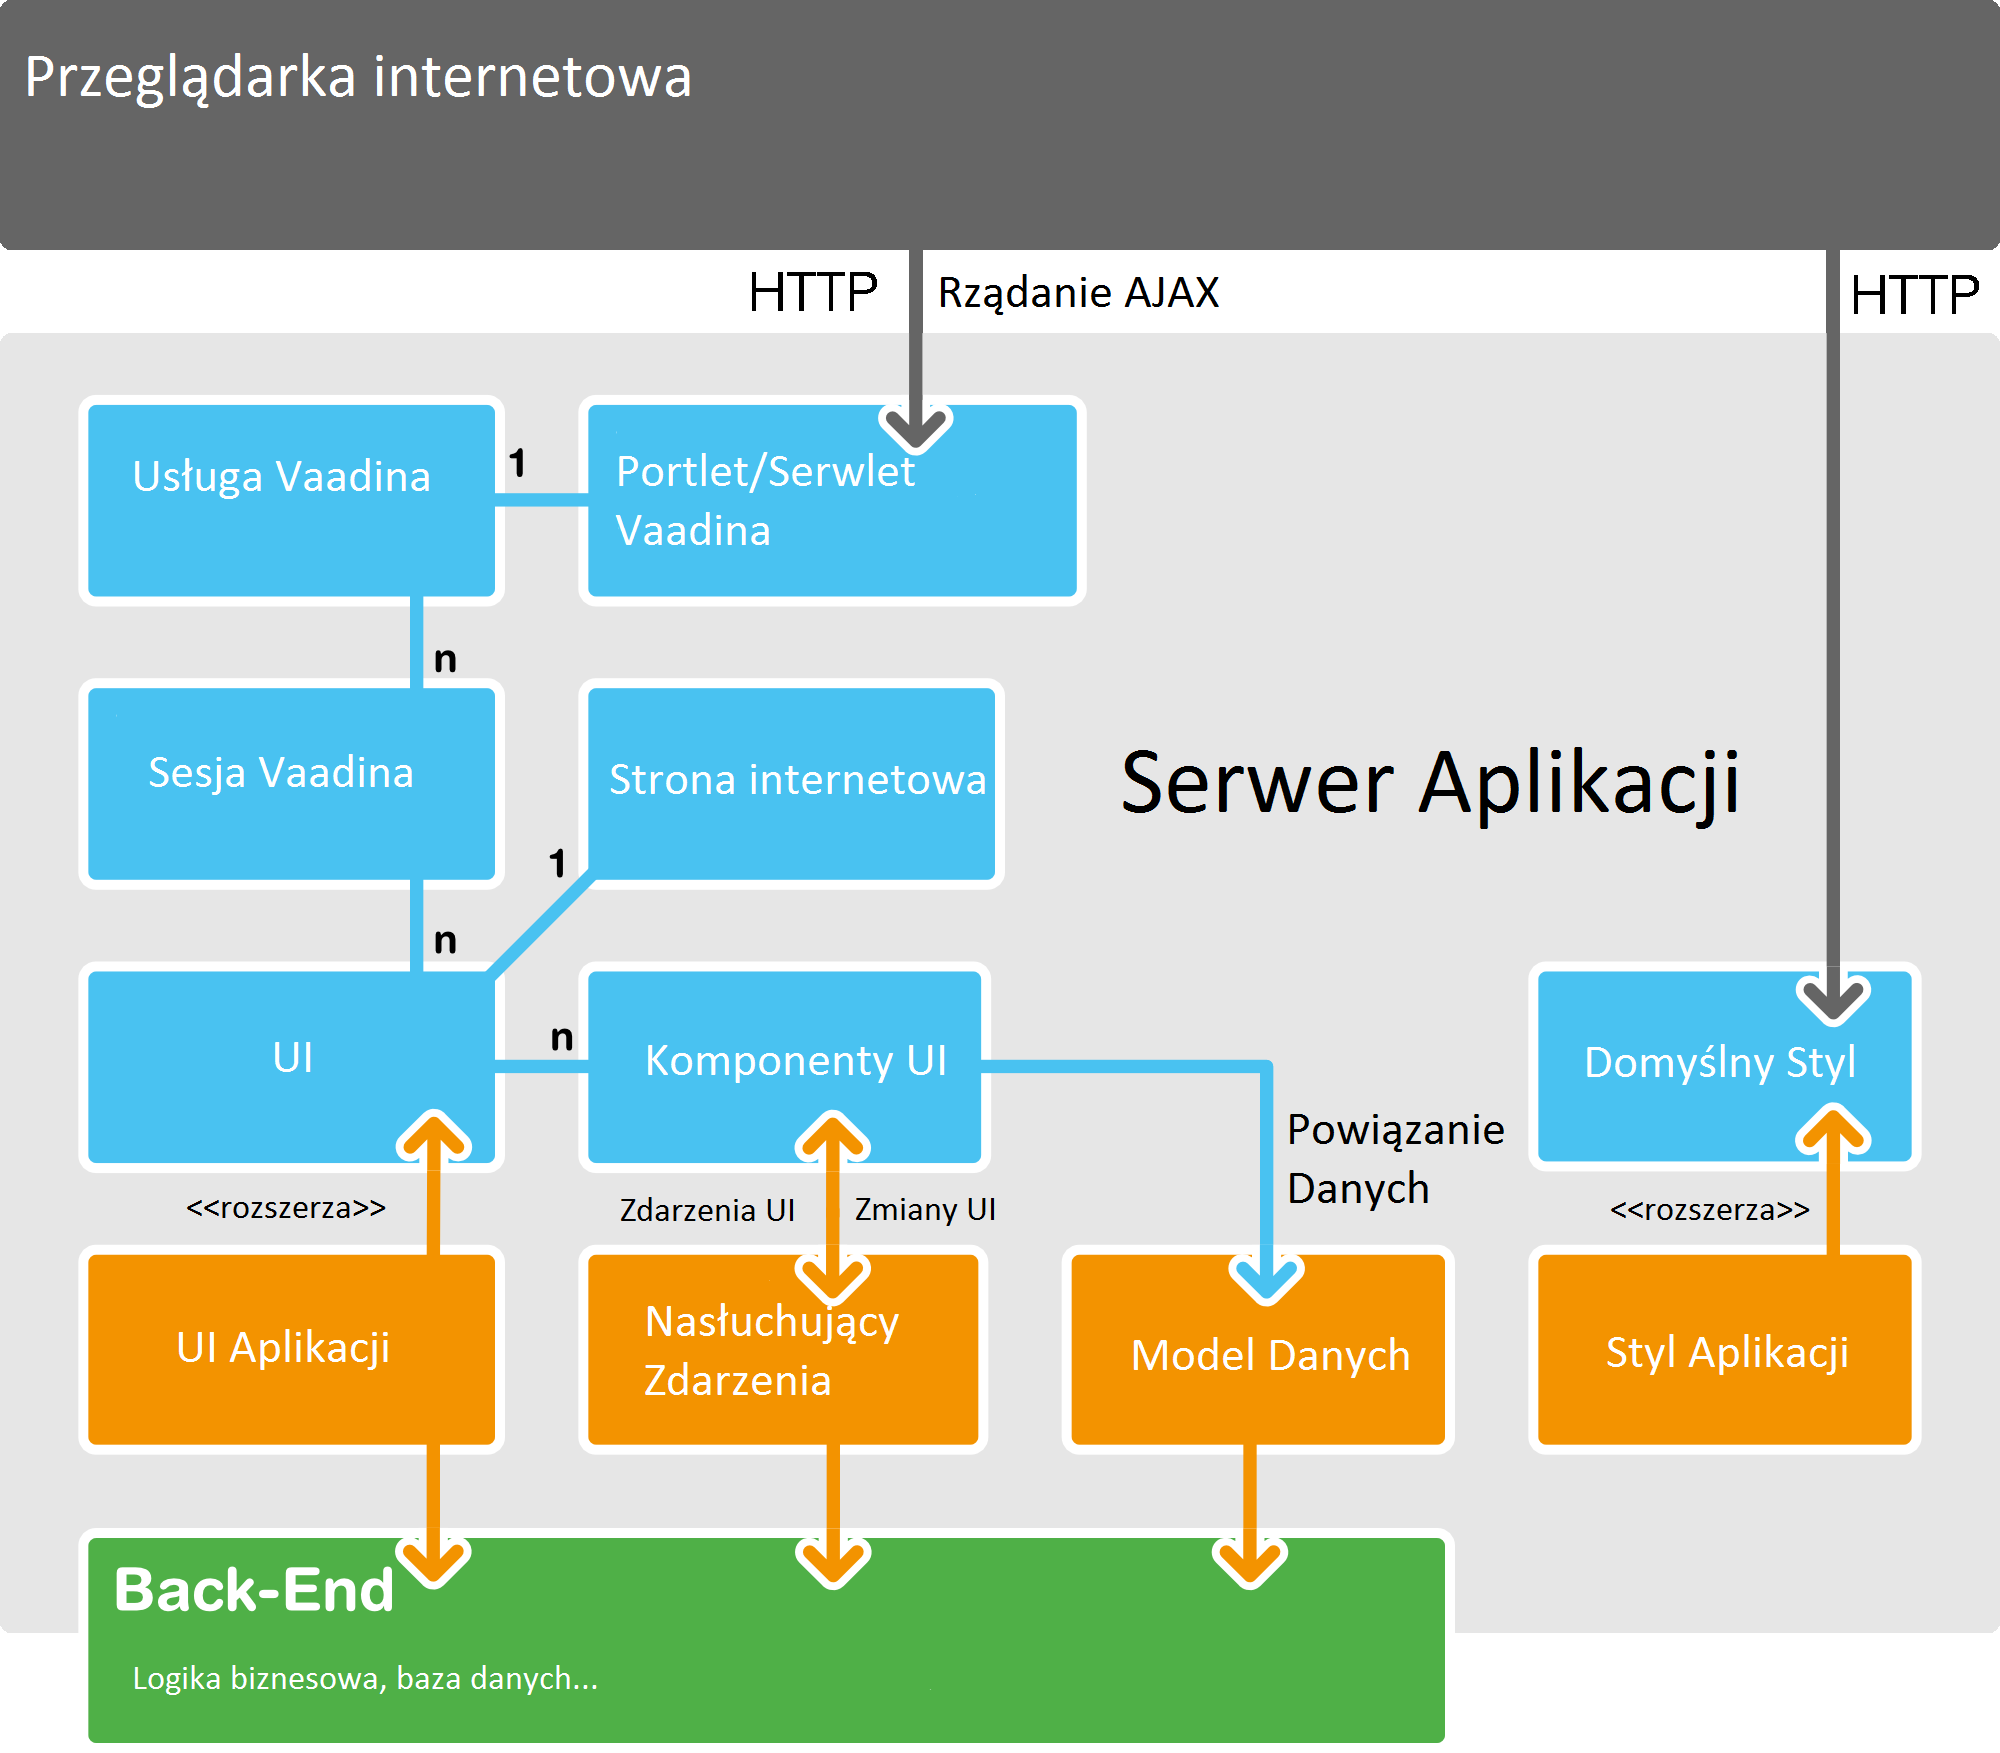
\includegraphics[scale=.3]{img/serverSide.png}
	\caption{Architektura szkieletu aplikacji Vaadin po stronie serwera}
	\label{serverVaadin}
    \end{center}
\end{figure}

\subsection{Zdalne wywoływanie procedury}
Cała tajemnica sukcesu Vaadin polega na zunifikowanym podejściu do obsługi zdarzeń. Każda kontrolka posiada swój łącznik, który jest podłączony do obiektu ApplicationConnection (jedna instancja na aplikacje) który odpowiada za komunikacje z serwerem po stronie klienta. Z drugiej strony natomiast występuje swego
rodzaju lustrzane odbicie – obiekt CommunicationManager jest połączony z każdym z komponentów. 

\begin{figure} [H]
    \begin{center}
	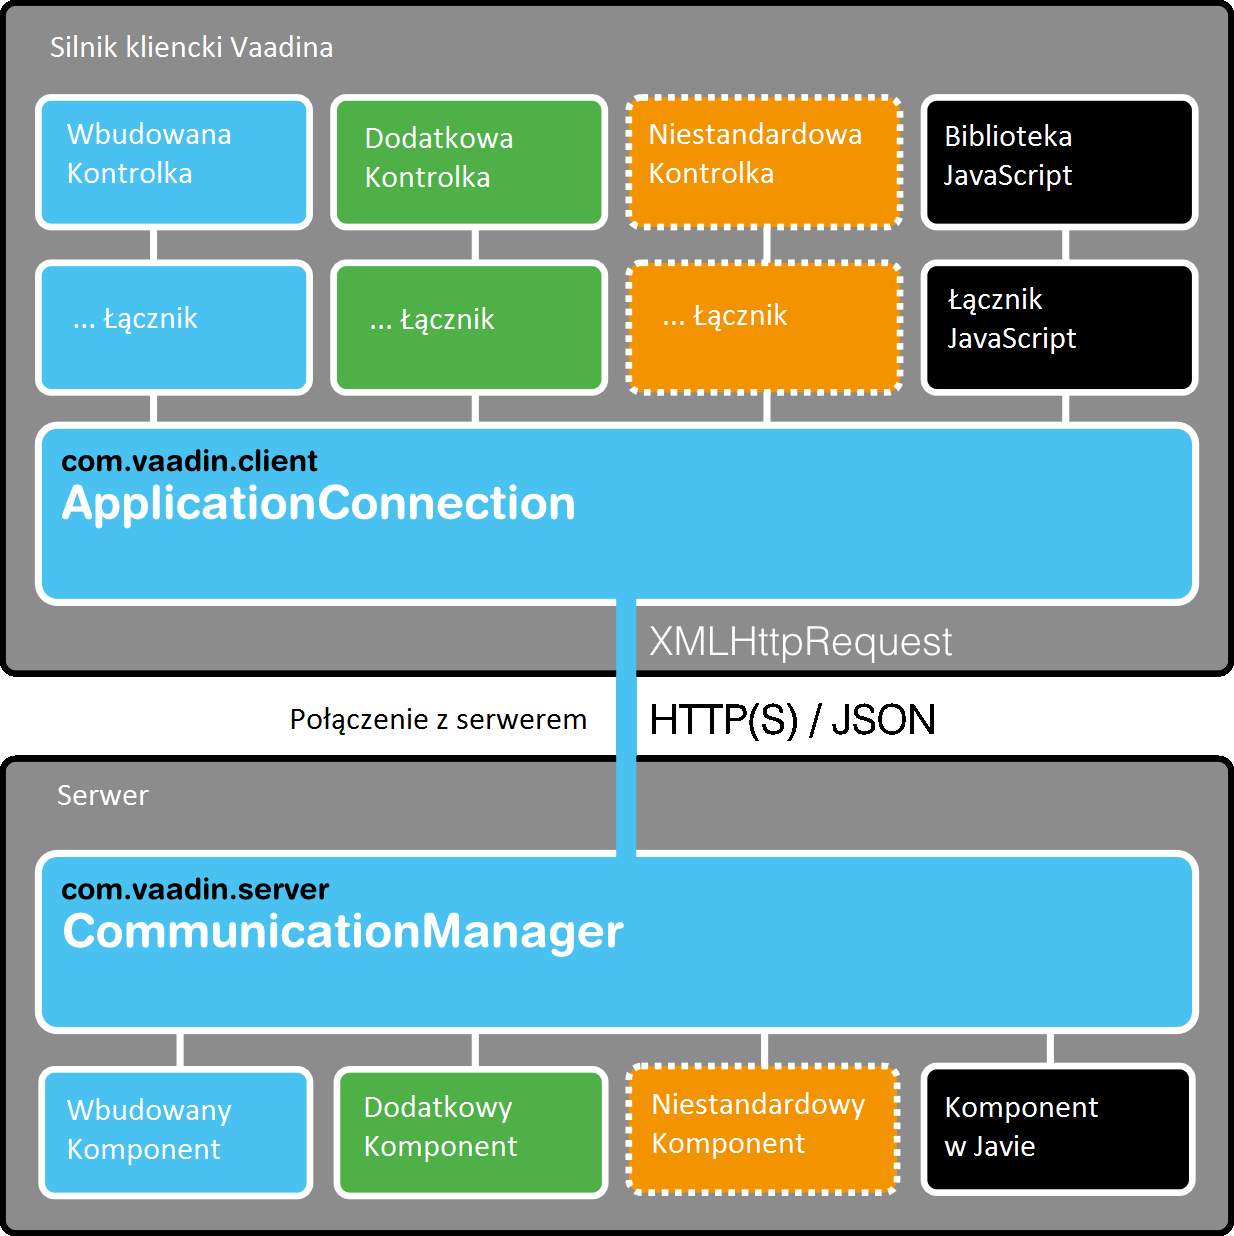
\includegraphics[scale=.3]{img/client.png}
	\caption{Komunikacja między kontrolką a komponentem}
	\label{architekturaVaadin}
    \end{center}
\end{figure}

Efekt ten można uznać za odmianę zdalnego wywoływania procedury – tzn. kontrolka wykonuje akcje związaną z nią przez JavaScript (jest to przezroczyste dla programisty) – komunikuje się przez WebService z serwletem Vaadina, który obsługuje żądanie, i w zależności od rezultatu – albo wysyła nową stronę do klienta albo asynchronicznie zmienia zawartość aktualnej.

\subsection{Architektura}
Do tej pory nie zostało to jeszcze powiedziane w sposób jednoznaczny – każdej kontrolce którą widzi użytkownik przyporządkowany jest po stronie serwera jeden komponent, który przechowuje stan kontrolki a także potrafi obsługiwać zdarzenia przez nią wygenerowane. 

\begin{figure} [H]
    \begin{center}
	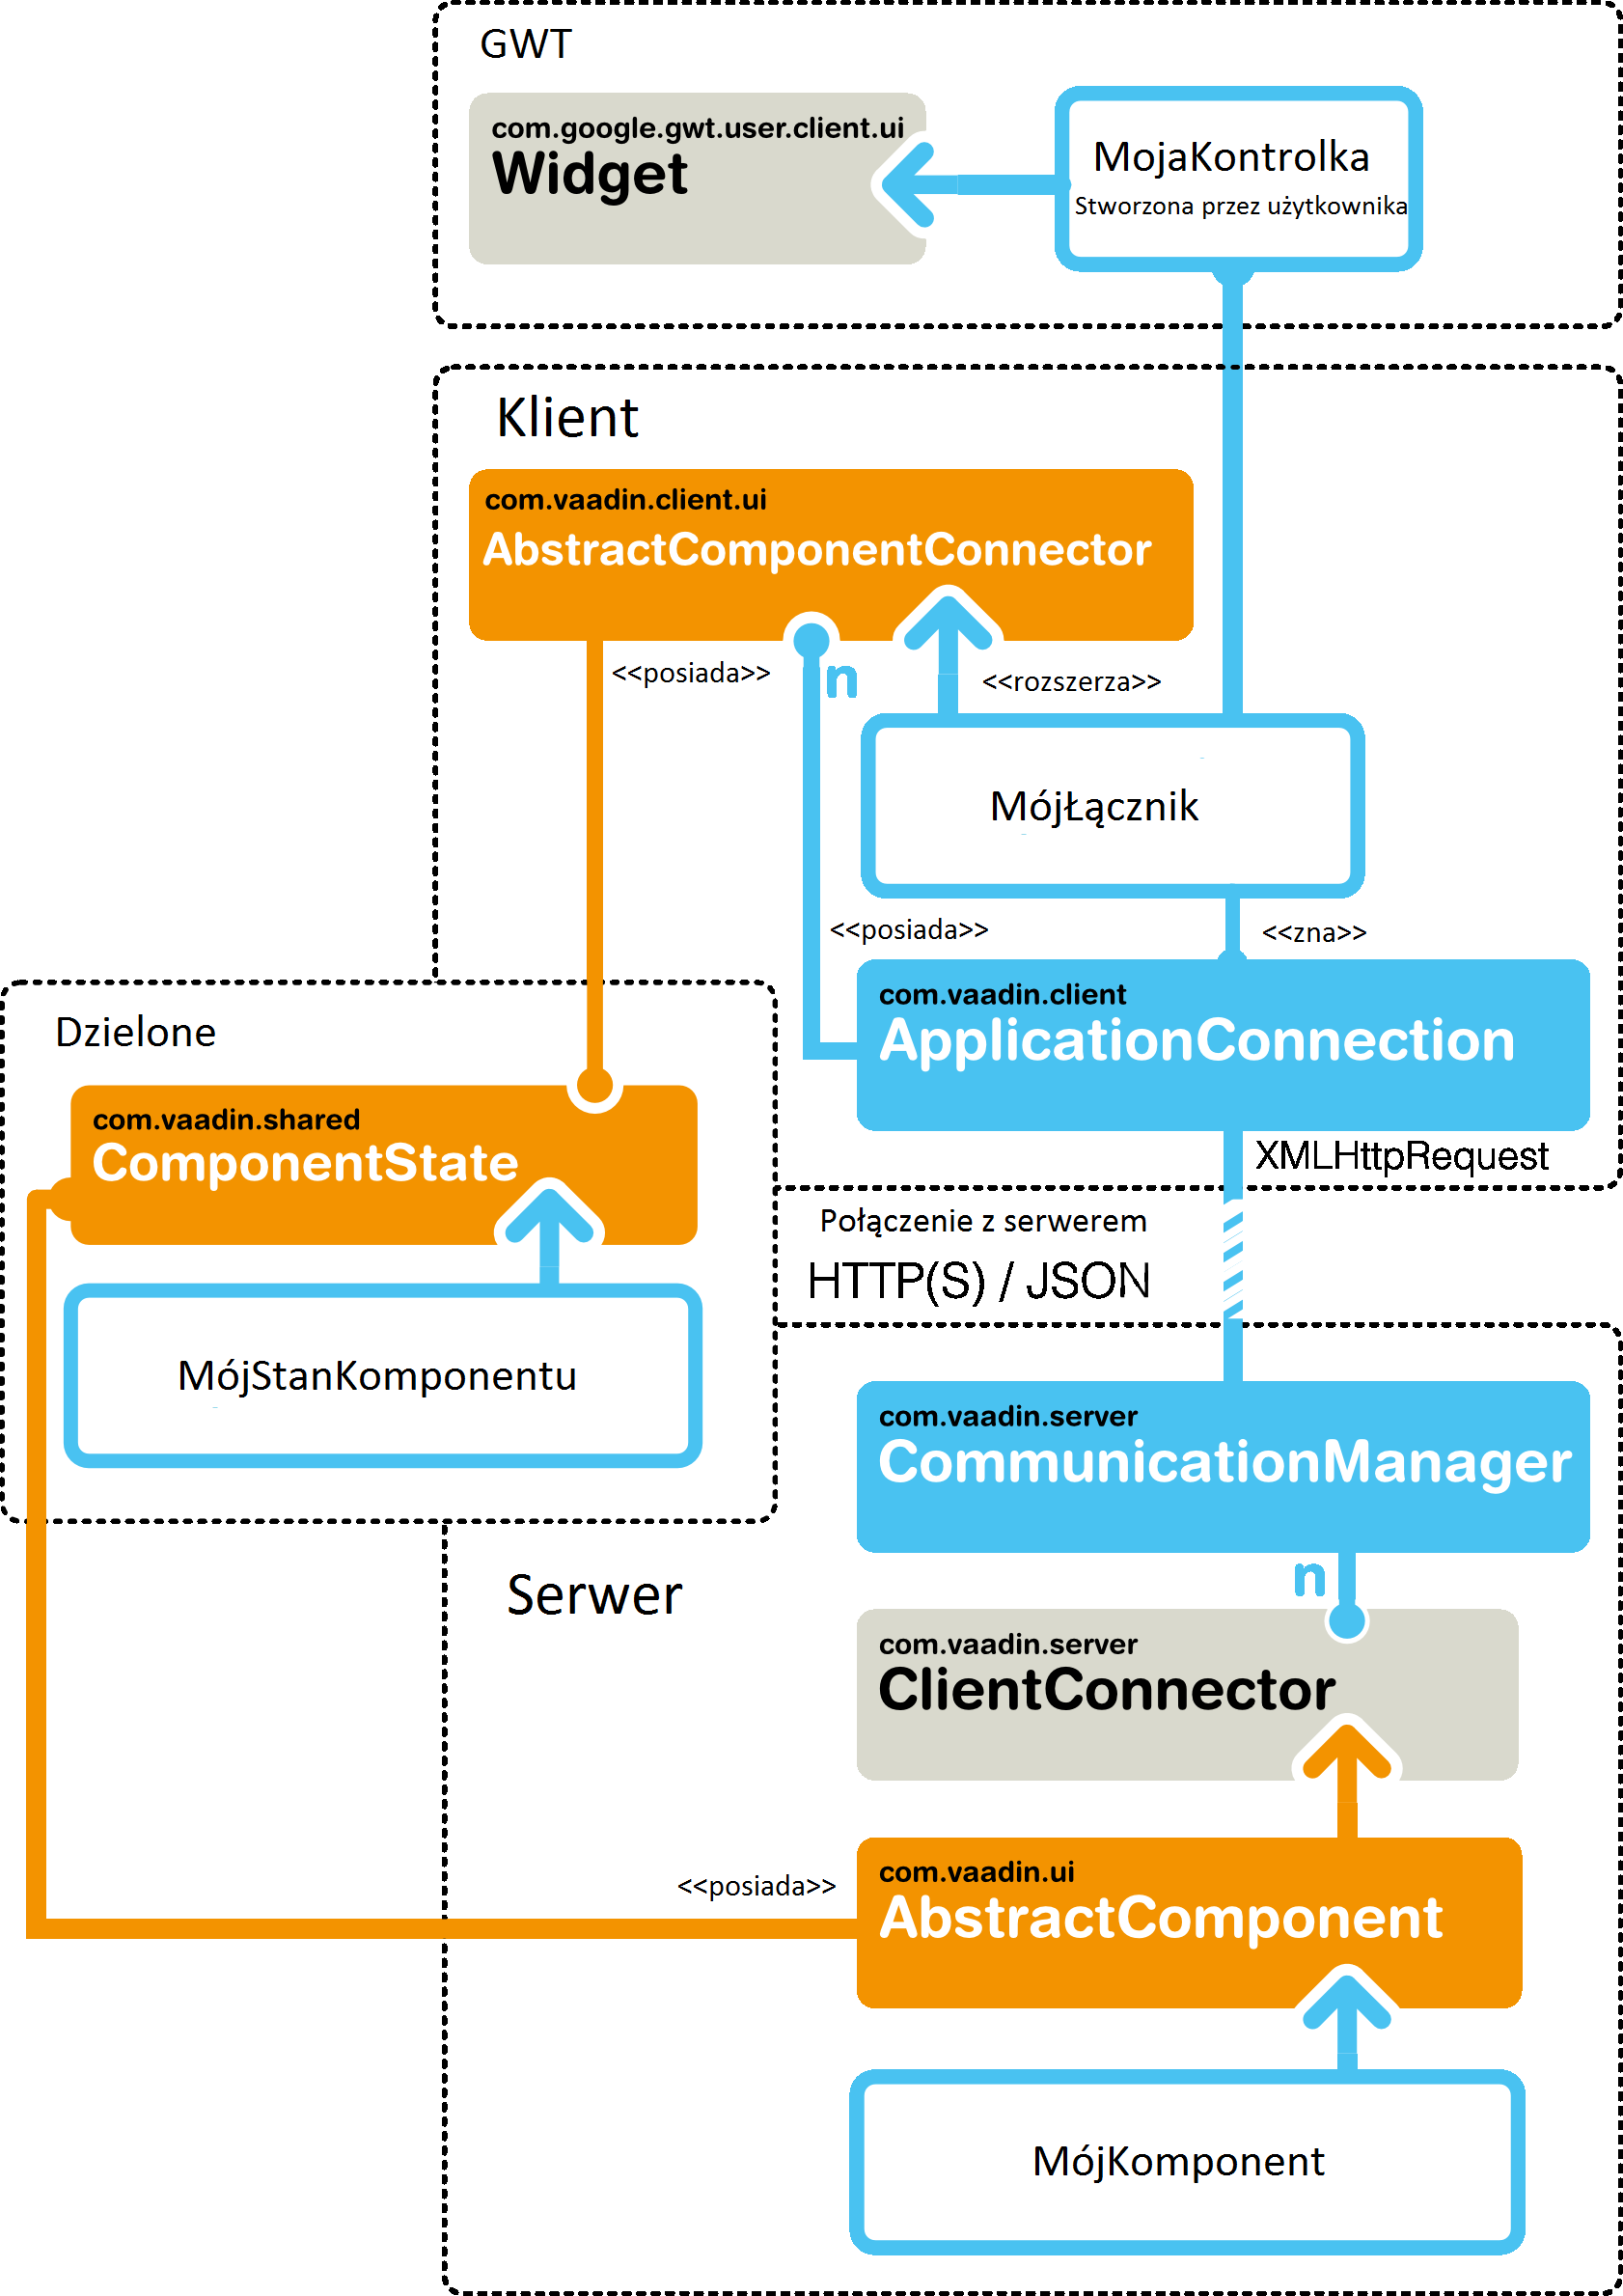
\includegraphics[scale=.2]{img/architektura.png}
	\caption{Implementacja połączenia kontrolki i komponentu}
	\label{clientVaadin}
    \end{center}
\end{figure}

Na powyższym schemacie przedstawiony jest sposób realizacji opisanego wcześniej podejścia. Z każdą kontrolką widzianą przez użytkownika związane są cztery klasy:
\begin{itemize}
\item Kontrolka – dziedzicząca po klasie Widget, definiująca co użytkownik widzi
\item Łącznik – który odpowiedzialny jest za przesyłanie informacji o zaistniałym zdarzeniu do serwera i synchronizacji stanu kontrolki
\item Komponent – klasa realizująca serwerową logikę kontrolki – realizuje reakcje na wygenerowanie zdarzenia, aktualizuje stan
\item Stan – klasa zawierająca informacje o aktualnym stanie kontrolki. 
\end{itemize}

Gdy zostanie wygenerowane zdarzenie przez kontrolkę po stronie klienta, łącznik przekazuje informacje o tym na stronę serwera do komponentu, który reaguje na tę zmianę. Możliwa jest zmiana stanu zarówno własnej kontrolki jak i innych kontrolek. Każdorazowa zmiana którejś z właściwości w obiekcie stanu powoduje asynchroniczną aktualizacje po stronie klienta.

\newpage
\subsection{Aplikacja po stronie klienta}
Jako jedną z zalet Vaadina zostało wymienione, że całość logiki znajdowała się po stronie serwera. Twórcy szkieletu aplikacji Vaadin zdają sobie jednak sprawę z tego, że część aplikacji potrzebuje natychmiastowych odpowiedzi (czyli nie ma czasu na czasochłonną komunikacje z serwerem przy każdym np. wciśnięciu klawisza) dlatego część zdarzeń powinna być obsługiwana po stronie klienta. 

Bardzo pomocny w tym celu okazuje się fakt, że Vaadin został stworzony jako obudowa dla GWT (Google Web Toolkit). Okazuje się, że istnieje możliwość skorzystania z kontrolek Google Web Toolkit w ramach aplikacji (istnieje także grupa kontrolek Vaadina dedykowanych specjalnie do tego rodzaju problemu).

\subsection{Nowe kontrolki}
Wielką zaletą szkieletu aplikacji który wybrałem jest spora liczba kontrolek będących w standardowym zestawie. Jeżeli jednak okazałoby się, że zbiór ten nie zawiera takiej, która jest potrzebna do zrealizowania funkcjonalności, warto udać się pod adres https://vaadin.com/download, pod którym do tej pory zostało opublikowanych prawie 400 nowych. 

Oczywiście może się okazać, że i w tej liście nie znajduje się odpowiednia kontrolka – w tym przypadku nie pozostaje już nic innego jak stworzyć nową. W ramach szkieletu aplikacji można tworzyć 4 rodzaje nowych kontrolek:
\begin{itemize}
\item Kontrolka złożona – składającą się z kilku istniejących kontrolek
\item Kontrolka rozszerzająca istniejącą (Vaadin) – zmieniająca właściwości / zachowanie tej kontrolki – np. zmiana tła pola tekstowego na niebieski
\item Kontrolka rozszerzająca istniejącą (GWT) – zaimplementowanie własnej kontrolki na podstawie istniejącej kontrolki z GWT
\item Całkiem nowa kontrolka, oparta o JavaScript/HTML – zaimplementowanie nowej kontrolki od zera również jest możliwe (choć skomplikowane).
\end{itemize}

\subsection{Style}
Ludzie którzy tworzyli strony internetowe z wykorzystaniem HTML mogą być przyzwyczajeni do możliwości wyprowadzania elementów dotyczących wyglądu aplikacji poza zawartość kodu strony (CSS). Twórcy Vaadina prawdopodobnie dostrzegli dużą zaletę w tego typu podejściu, ponieważ w tym szkielecie aplikacji również jest to możliwe. Mechanizm ten jest wierną kopią kaskadowych arkuszy styli – można określać styl na każdym poziomie aplikacji, jednocześnie przykrywając go na poziomie niżej, np. kod powoduje że wszystkie tła w aplikacji będą koloru żółtego:
\newpage
\begin{lstlisting}
.v-app {
	background: yellow;
}
\end{lstlisting}
Natomiast dopisując poniższy kod uzyskiwany jest efekt, polegający na tym że wszystko oprócz przycisków będzie posiadać żółte tło, które będą mieć tło kolorowane na niebiesko:

\begin{lstlisting}
.v-app .mybutton {
	background: blue;
}
\end{lstlisting}
\subsection{Powiązanie danych}
Główną rolą aplikacji internetowych jest przetwarzanie informacji. Ważnym elementem jest wyświetlanie danych wprowadzonych do bazy do tej pory, potrzebne jest także umożliwienie edycji / dopisania / usunięcia elementu. Tak samo jak każdy szanujący się szkielet aplikacji, Vaadin umożliwia uproszczenie tego procesu za pomocą powiązania danych (ang. Data Binding). W Vaadinie istnieją trzy wymiary, w których przechowywane są dane:
\begin{itemize}
\item Właściwość (ang. Property) – każda kontrolka posiada przypisaną do niej właściwość
\item Pozycja (ang. Item) – każdy formularz lub wiersz w tabeli posiada odpowiadającą mu pozycję
\item Pojemnik (ang. Container) – każdej tabeli odpowiada pojemnik przechowujący jej dane
\end{itemize}

Co daje powiązanie danych? Umożliwia to w prosty sposób edycje obiektów w bazie danych. Na przykład, wprowadzenie danych do formularza jest jednoznaczne z ustawieniem właściwości w obiekcie, dzięki czemu w wyniku np. kliknięcia przycisku dodaj, szkielet aplikacji dostarcza wypełniony już obiekt, gotowy do wprowadzenia do bazy danych. 

Innym przykładem korzyści płynących z powiązania danych jest usunięcie wiersza z tabeli. Dzięki temu mechanizmowi minimalozowana jest praca polegająca na oprogramowywaniu przycisku usuń.

Ważnym elementem, w kontekście powiązania danych jest proces walidacji danych (szczególnie w formularzu). Vaadin umożliwia (jak większość szkieletów aplikacji) sprawdzenie poprawności wprowadzonych informacji, i w razie potrzeby wyświetla potrzebną informacje zwrotną o błędzie użytkownikowi. Walidacja odbywa się zgodnie ze standardem Java Bean Validation (JSR-303).
\newpage
\section{Podsumowanie}
Wybrane przez autora technologie zostały dopasowane do potrzeb tworzonego systemu, ponieważ w pracy nad każdym oprogramowaniem do wyboru narzędzi wspierających budowę powinno się podchodzić indywidualnie.

Należy także pamiętać, że technologie użyte przez autora do stworzenia systemu będącego tematem pracy, nie są uniwersalne - a wręcz przeciwnie - były aktualne i dosyć powrzechne w chwili pisania tej pracy. Bardzo prawdopodobne jest jednak, że za kilka lat zostaną uznane w środowisku informatycznym za przestarzałe, a w ich miejsce powstaną nowe, lepsze i/lub wydajniejsze.

% ex: set tabstop=4 shiftwidth=4 softtabstop=4 noexpandtab fileformat=unix filetype=tex spelllang=pl,en spell: